\begin{enumerate}
    \item Se diseña un filtro que tiene dos ceros conjugados sobre el círculo unitario en un ángulo $\theta$ en el plano $\mathcal{Z}$. Se deben agregar dos polos para que el sistema sea causal, por lo que se escogen dos polos en $z = 0$ ya que no afectan la respuesta del filtro.
    
    $$ H(z) = \frac{(z- e^{j \theta})(z-e^{-j \theta})}{z^2} = \frac{z^2 - 2~z~cos(\theta)+ 1}{z^2}$$
    
    De donde se obtiene  la ecuación de diferencias 
    
    $$ y[n] = x[n] -2~cos(\theta )~ x[n-1] + x[n-2]$$
    
    
        Se estudia  la respuesta  a impulso de este filtro para valores de $ \theta = \left \lbrace \pi/6,~ \pi/3,~\pi/2 \right \rbrace$, el resultado obtenido se muestra en las gráficas de la figura \ref{resp_impuilso}
        
        \begin{figure}[H]
            \centering
            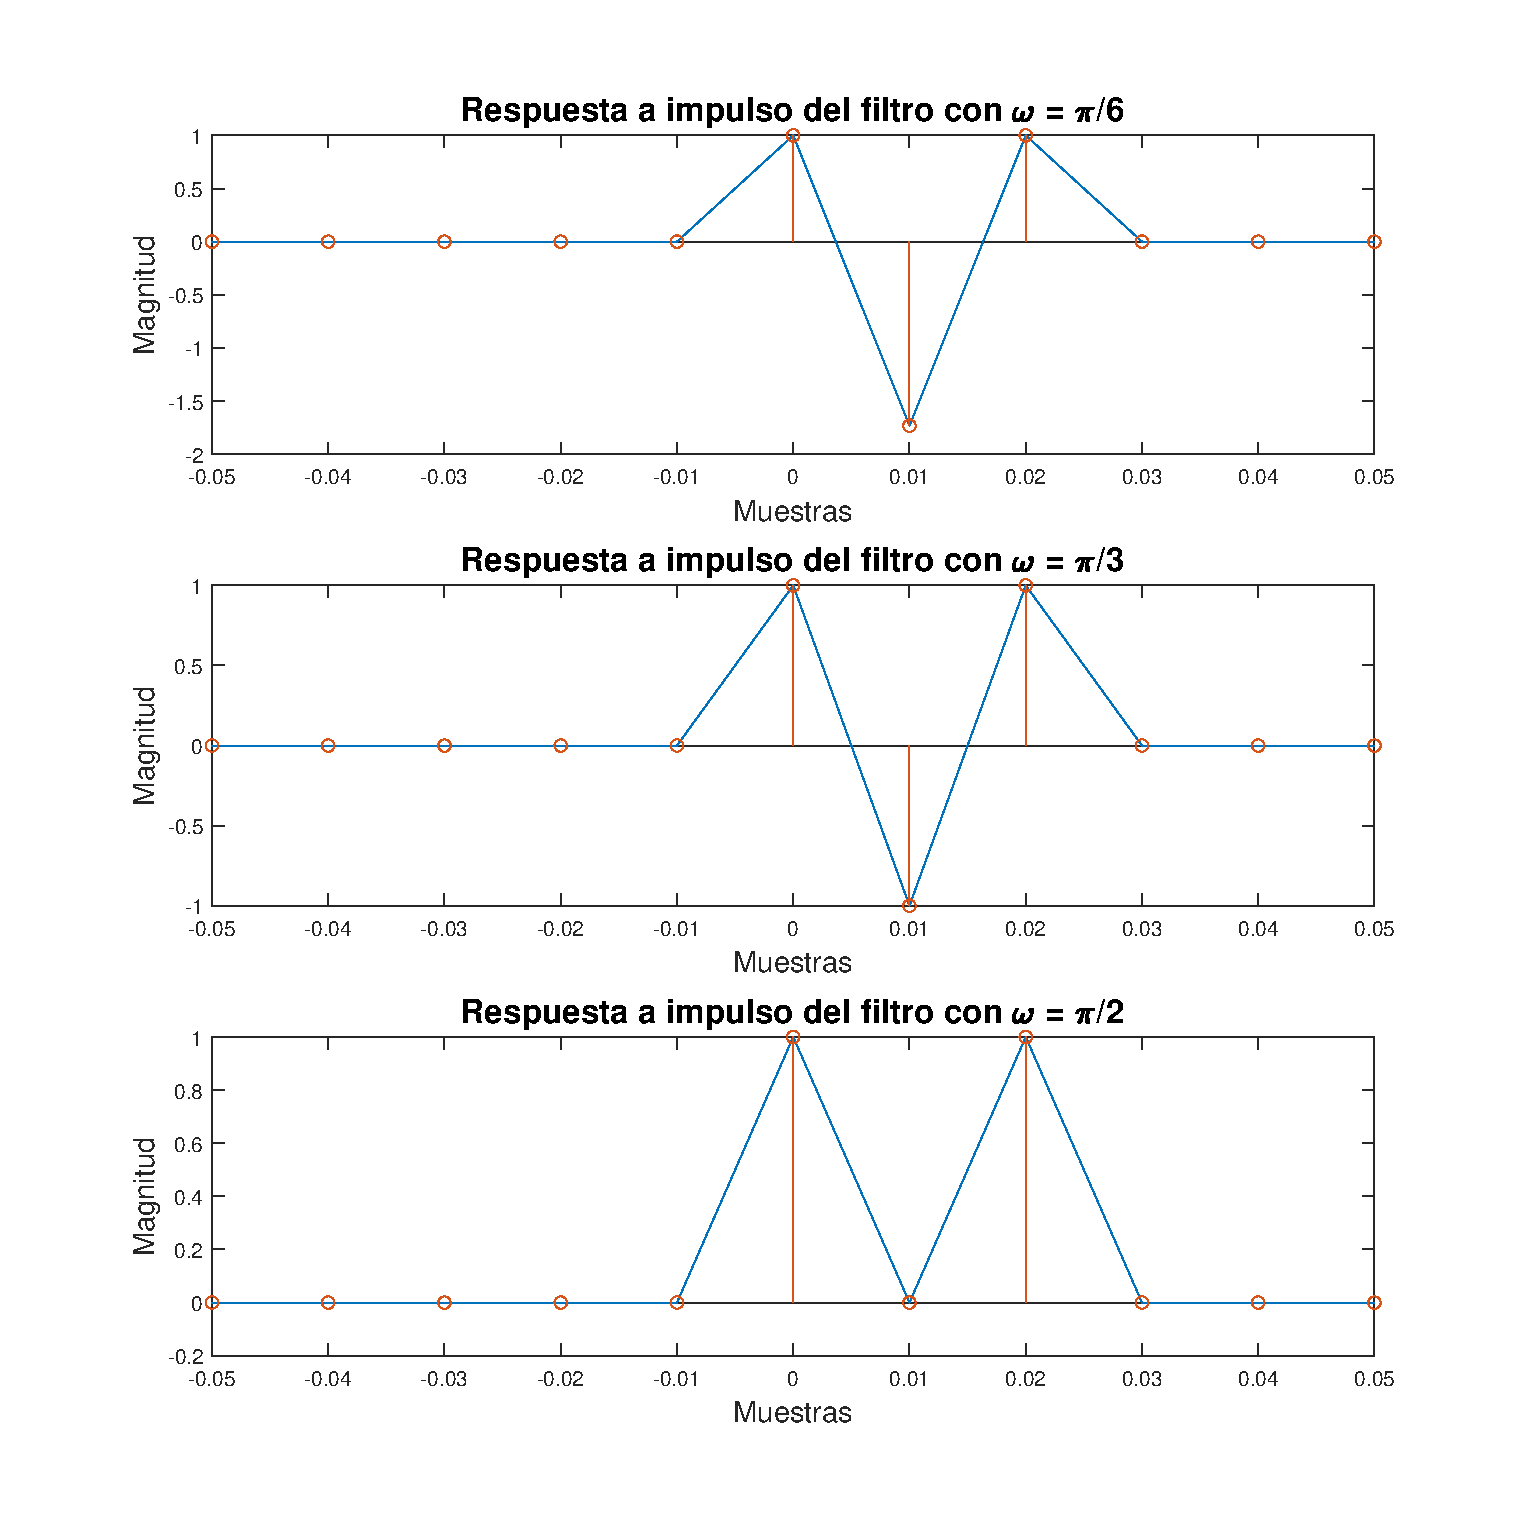
\includegraphics[scale = 0.5]{Figuras/p1_1-Respuesta_impulso.eps}
            \caption{Respuesta impulso del filtro para ángulos $ \theta = \left \lbrace \pi/6,~ \pi/3,~\pi/2 \right \rbrace$}
            \label{resp_impuilso}
        \end{figure}
    
    
    Haciendo el reemplazo de $z = e^{jwT_s}$ se puede obtener una expresión analítica para la función de transferencia del filtro diseñado en función de la frecuencia $\omega$.
    
        $$ H(z) = \frac{e^{2 j \omega T_s} - 2~e^{j \omega T_s}~cos(\theta)+ 1}{e^{2 j \omega T_s}}$$
    

    
    Se obtiene la respuesta en frecuencia del filtro diseñado  en función del ángulo para   $ \theta = \left \lbrace \pi/6,~ \pi/3,~\pi/2 \right \rbrace$   de donde tienen como resultado las gráficas de la figura \ref{frec_resp}
    
\begin{figure}[H]
    \centering
    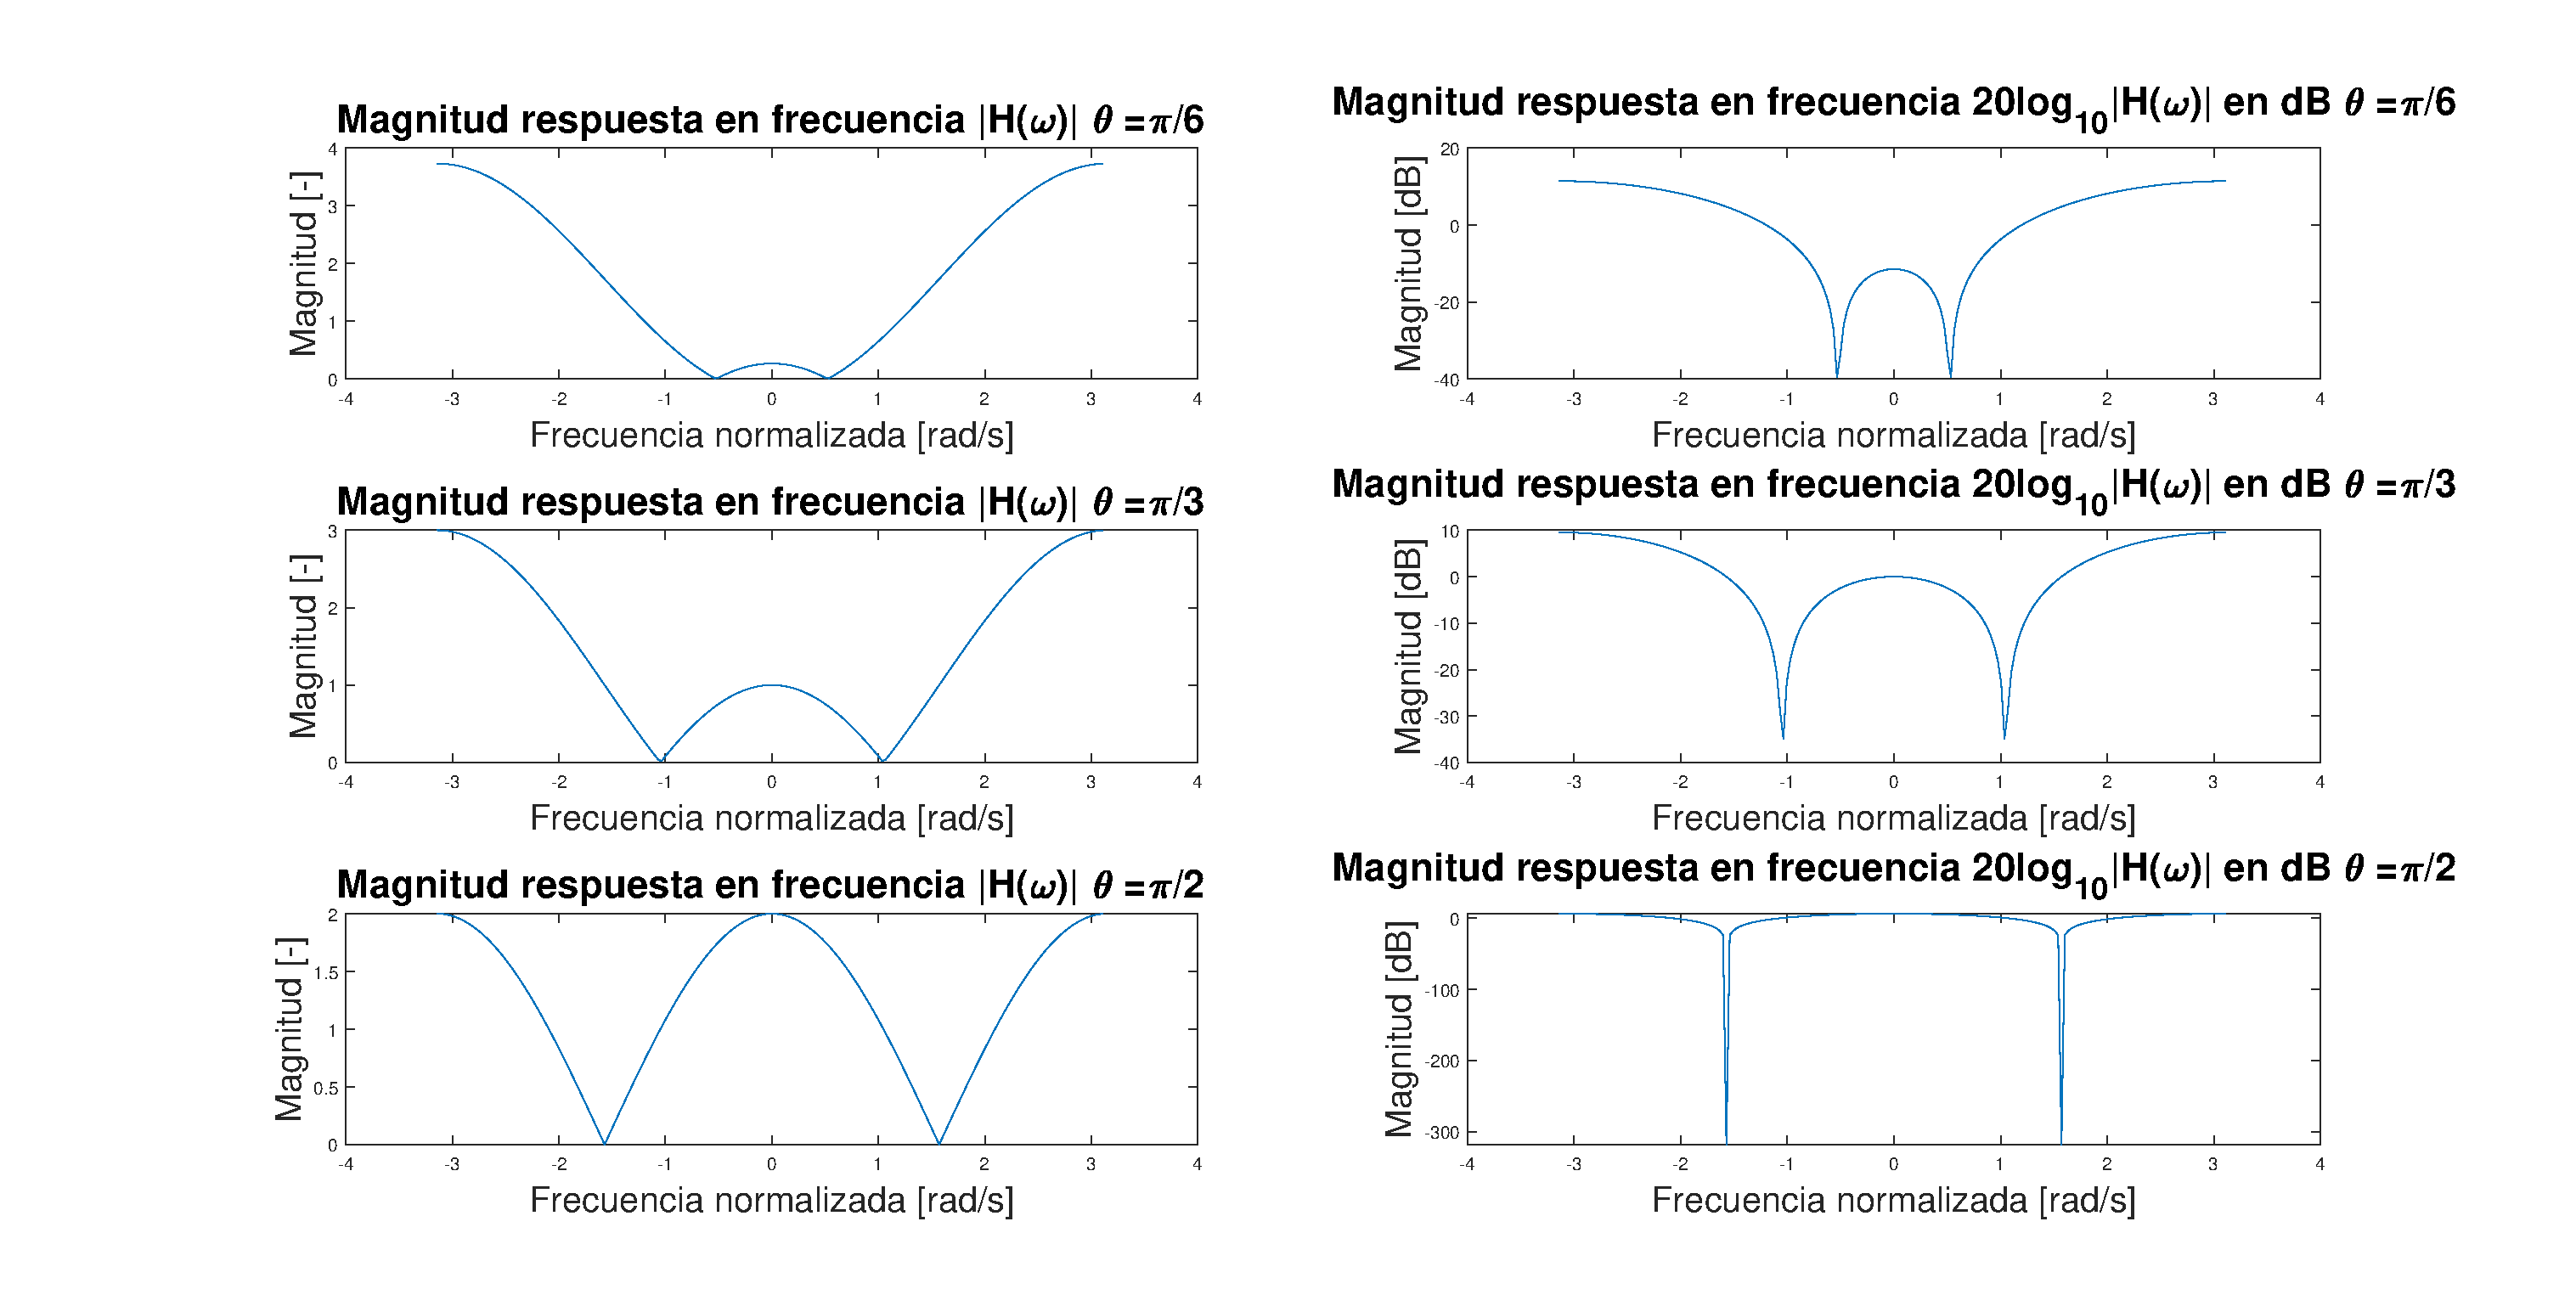
\includegraphics[scale = 0.3]{Figuras/p1_1-Respuesta_en_frecuencia.eps}
    \caption{Respuesta en frecuencia del filtro diseñado para  $ \theta = \left \lbrace \pi/6,~ \pi/3,~\pi/2 \right \rbrace$ }
    \label{frec_resp}
\end{figure}
    
    
    
    En la figura \ref{frec_superpuesta} se pueden observar las gráficas asociadas a los tres ángulos probados de manera superpuesta observar el efecto del ángulo en la respuesta en frecuencia del filtro.
    
    \begin{figure}[H]
        \centering
        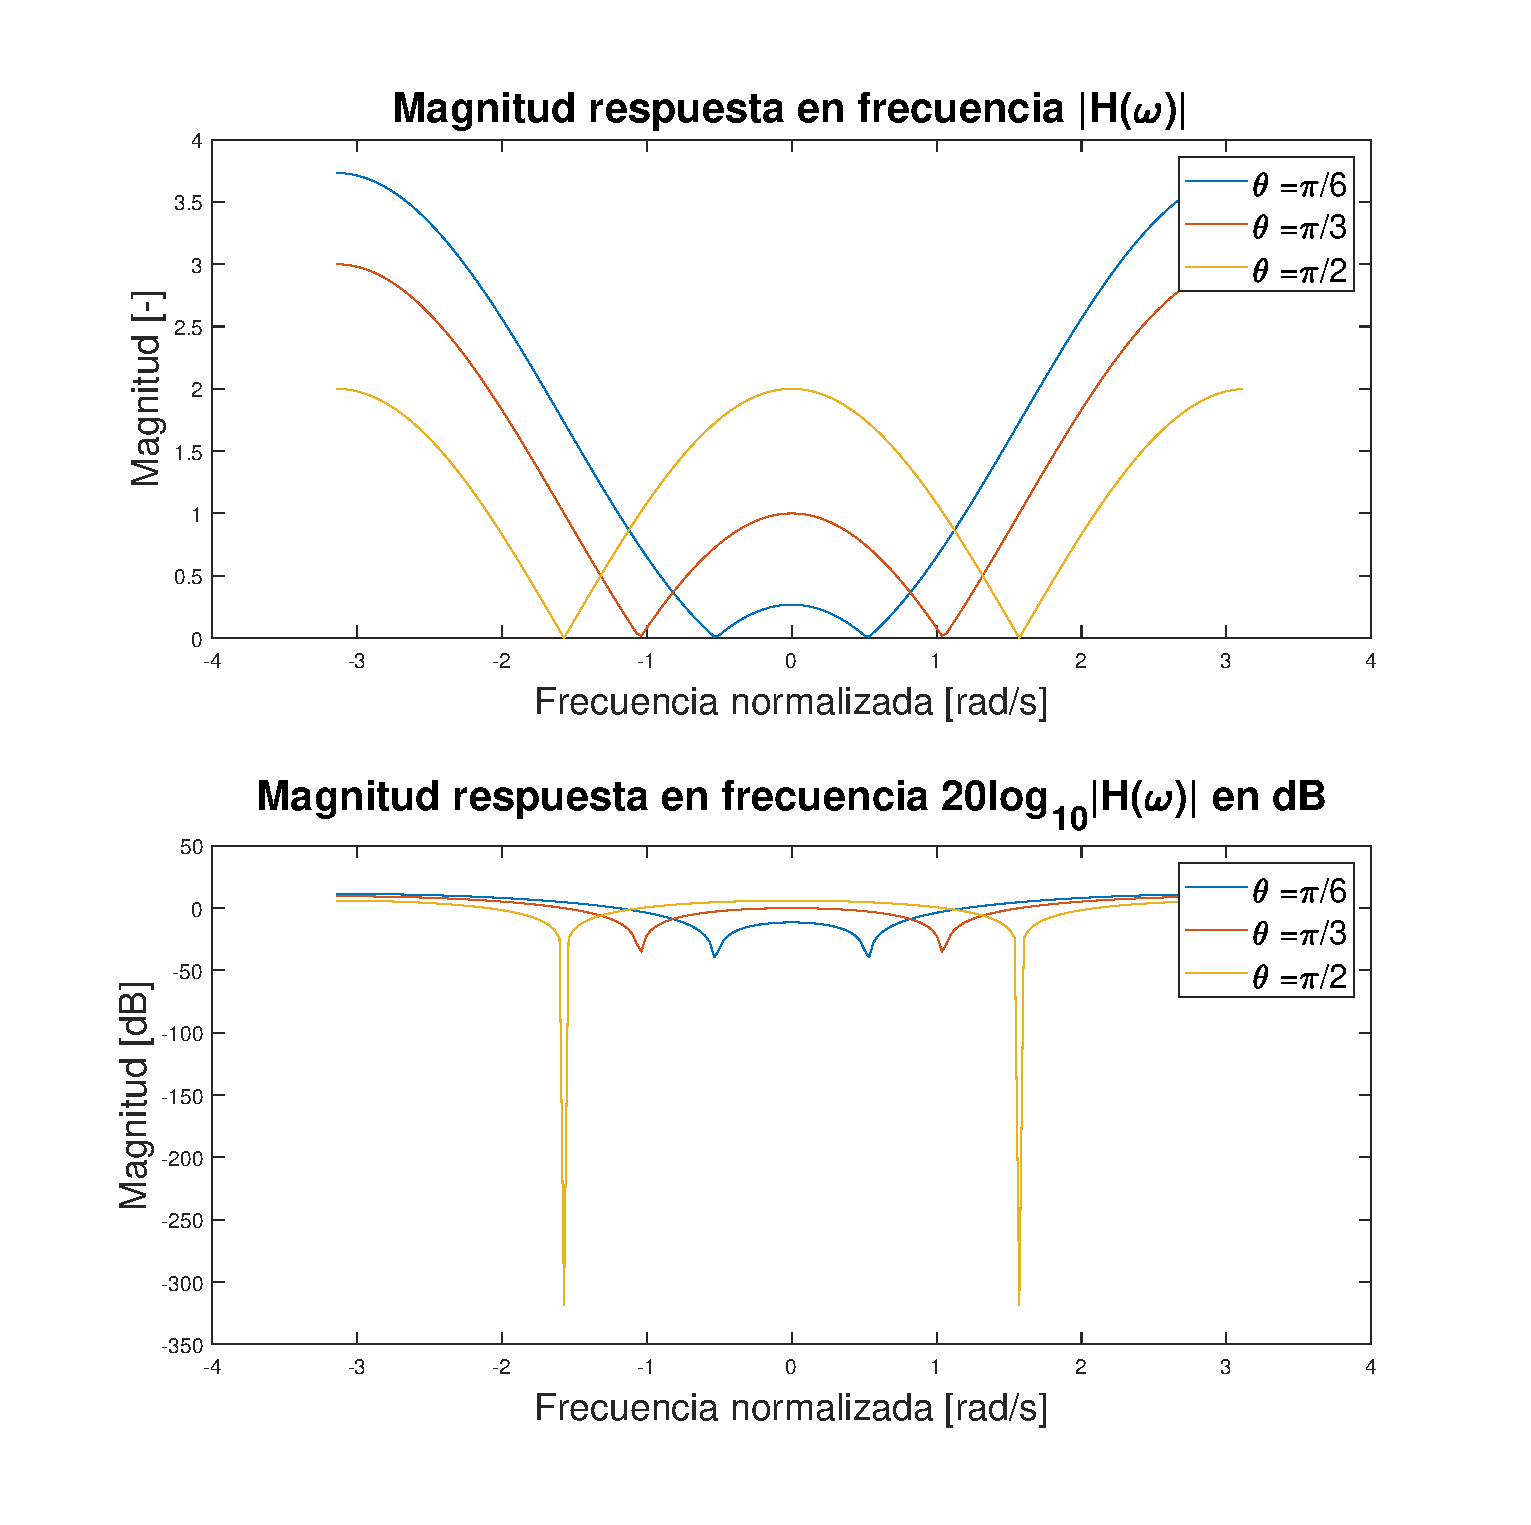
\includegraphics[scale = 0.4]{Figuras/p1_1-Respuesta_superpuesta.eps}
        \caption{Respuestas en frecuencia superpuestas del filtro diseñado para $ \theta = \left \lbrace \pi/6,~ \pi/3,~\pi/2 \right \rbrace$}
        \label{frec_superpuesta}
    \end{figure}
    


De las gráficas anteriores se puede ver como la frecuencia en la que la magnitud en frecuencia se hace cero, en una gráfica respecto a la frecuencia normalizada, corresponde justamente al valor de $\theta$, ya que para el conjunto de valores probados  $ \theta = \left \lbrace \pi/6,~ \pi/3,~\pi/2 \right \rbrace$, la respuesta en frecuencia del sistema se hace cero en $ rad/s = \left \lbrace 0.5235,~ 1.0471,~1.5707 \right \rbrace$

 
La relación que existe entre el ángulo $\theta$ con la respuesta en frecuencia del filtro con una frecuencia de muestreo $fs$ esta dada por 
$$ \theta = \frac{2 \pi f}{fs}$$ 

Ya que existe la razón directa entre $2\pi$ que corresponde a una vuelta completa al circulo unitario en el plano $\mathcal{Z}$ al igual que $fs$. Por lo que de esta forma se puede normalizar el valor de  una  frecuencia dada y llevarlo a la variable $\theta$. Observando el gráfico de la figura \ref{frec_superpuesta}, se puede concluir también que el valor de $f$ en la expresión anterior corresponde al valor de la frecuencia de corte del filtro en $Hz$ y por consiguiente $\theta$ es la frecuencia de corte del filtro frecuencia normalizada medida en $rad/muestra$.

%Rodrigo%%%%%%%%%%%%%%%%%%%%%%%%%%%%%%%%%%%%%%%%%%%%%%%%%%%%%%%%%%
\item  Se diseña un filtro que tiene dos polos conjugados dentro del círculo unitario en un ángulo $\theta$ en el plano $\mathcal{Z}$, con ganancia $1-r$. La función de transferencia queda dada por
\begin{align}
   H(z) &= \frac{1-r}{(z- re^{j \theta})(z-re^{-j \theta})} = \frac{1-r}{z^2 - 2zr\cos(\theta)+ r^2}\nonumber\\
   &= \frac{(1-r)z^{-2}}{1 - 2rz^{-1}\cos(\theta)+ r^2z^{-2}}\label{p1_2_Hz}
\end{align}
    
De donde se obtiene  la ecuación de diferencias: 
    
$$ y[n] = (1-r)x[n-2] +2r\cos(\theta )y[n-1] - r^2y[n-2]$$
    
Posteriormente se grafican las respuestas impulso a partir de la ecuación de recurrencia, para $r$ = 0.99, 0.9, 0.7 y $\theta = \pi/3$. Los gráficos se muestran en la figura \ref{fig:p1_2_ri}. Notar que el decaimiento de las respuesta a impulso es más lento a medida que $r$ está mas cercano al circulo unitario, pues se acerca a la zona inestable, y que el factor sinusoidal de las 3 respuestas a impulso comparten frecuencia. 

\begin{figure}[H]
    \centering
    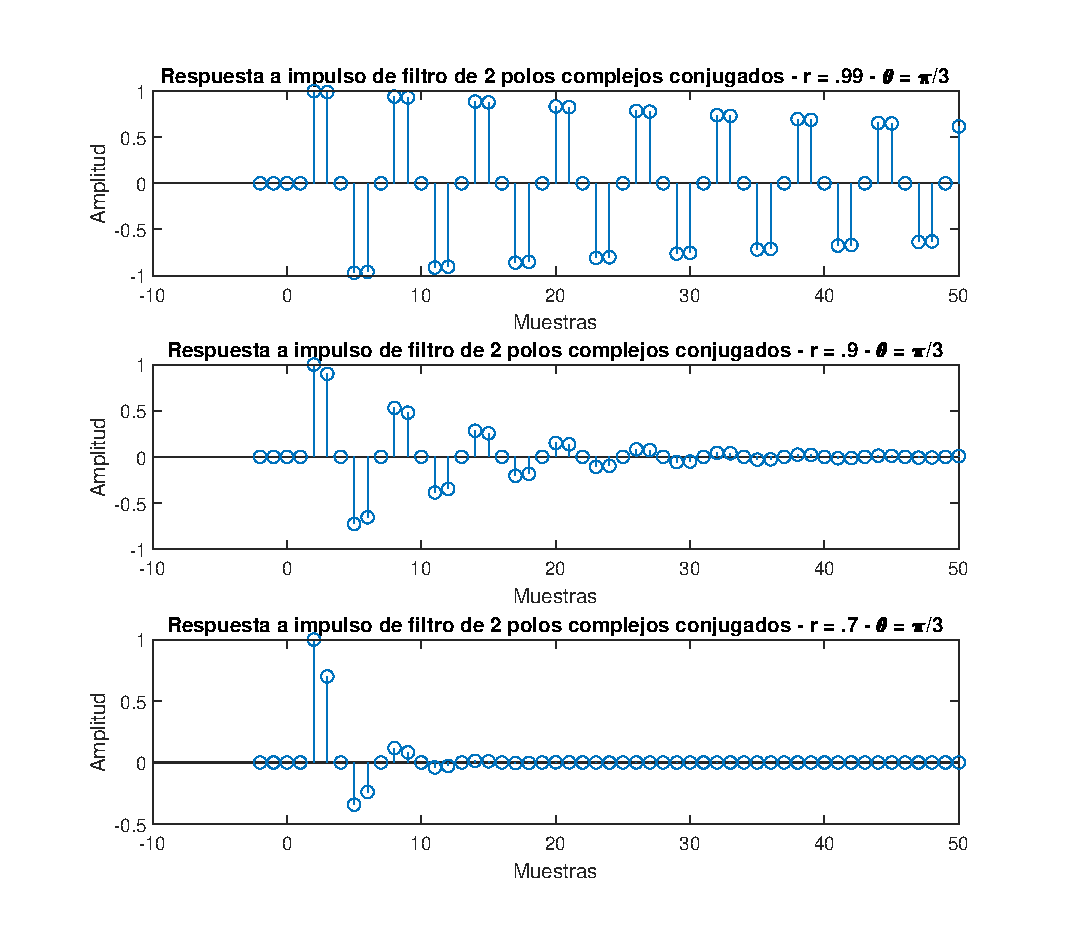
\includegraphics[width = .95\linewidth]{Figuras/p1_2_ri.eps}
    \caption{Respuestas a impulso de sistema de 2 polos complejos conjugados.}
    \label{fig:p1_2_ri}
\end{figure}

Luego, a partir de la función de transferencia (\ref{p1_2_Hz}) se obtiene la respuesta en frecuencia a partir de $H(z=e^{j\omega Ts})$, obteniendo:

$$ H(e^{j\omega Ts}) = \frac{1-r}{e^{2j\omega Ts} - 2ze^{j\omega Ts}\cos(\theta)+ r^2} $$

expresión que se usa para graficar las respuestas en frecuencia del filtro para $r$ = 0.99, 0.9, 0.7 y $\theta = \pi/3$. Las respuestas en frecuencia se muestran en la figura  \ref{fig:p1_2_rf}.

Notar que:
\begin{itemize}
    \item La frecuencia de resonancia se mantiene en $\theta = \tfrac{\pi}{3}$ para los 3 filtros.
    \item El peak es mayor a medida que $r$ a 1 , es decir, cuando los polos se acercan a la zona inestable.
    \item El filtro corresponde a un pasa banda el cual es mas selectivo (disminuye ancho de banda) a medida que $r$ crece
\end{itemize}

\begin{figure}[H]
    \centering
    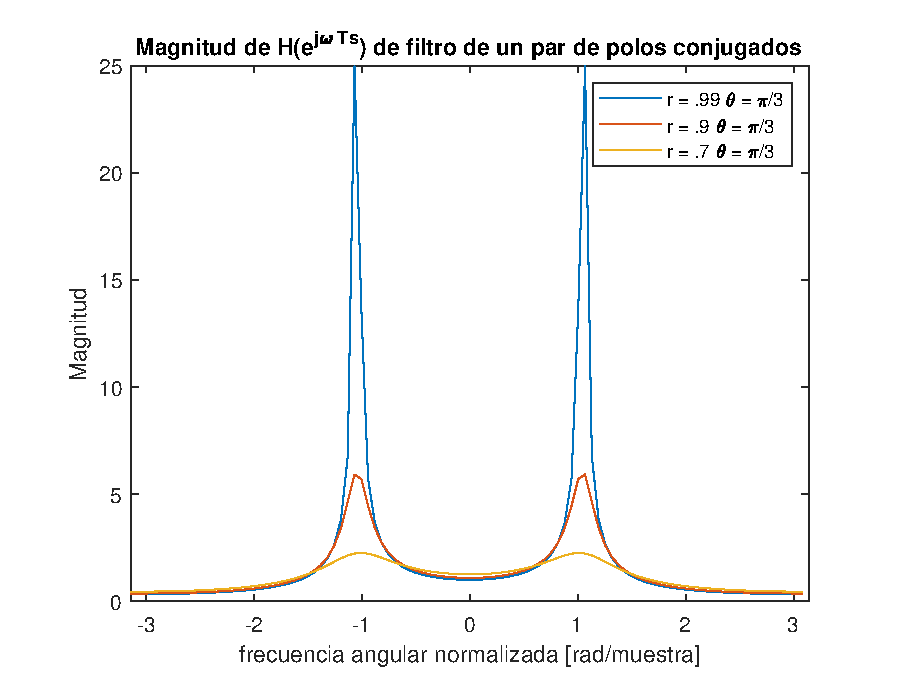
\includegraphics[width = .95\linewidth]{Figuras/p1_2_rf.eps}
    \caption{Respuestas en frecuencia de sistema de 2 polos complejos conjugados.}
    \label{fig:p1_2_rf}
\end{figure}
    
    

%%%%%%%%%%%%%%%%%%%%%%%%%%%%%%%%%%%%%%%%%%%%%%%%%%%%%%%%%%%%%%%%%%%
\item  Haciendo uso de la función  \texttt{DTFT.m} entregada en los recursos para el laboratorio se puede obtener el espectro en frecuencias correspondiente al archivo \texttt{nspeech.mat}, y identificar la frecuencia del tono puro presente en el archivo, como se ve en la figura \ref{nspeech_tone}

\begin{figure}[H]
    \centering
    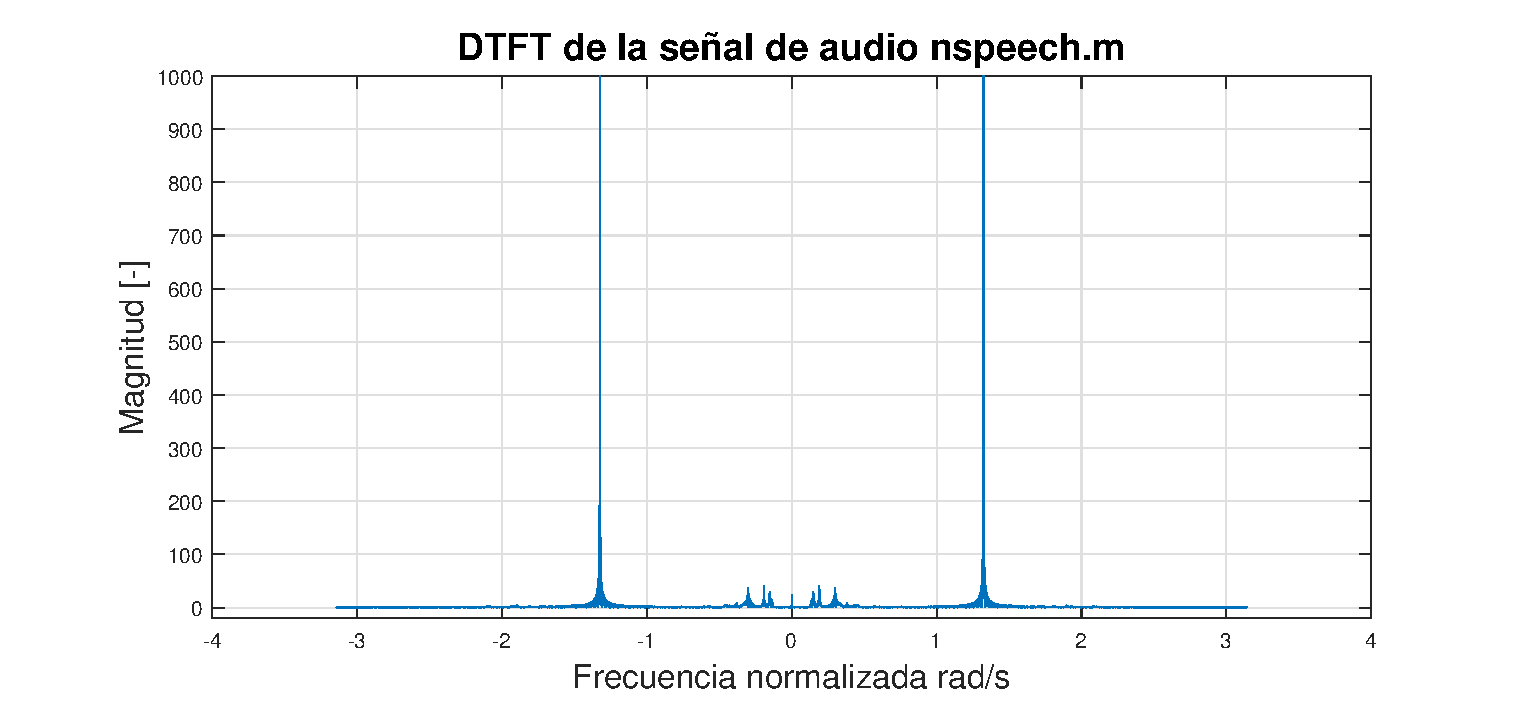
\includegraphics[scale = 0.6]{Figuras/p1_3-DTFT.eps}
    \caption{Espectro en frecuencia normalizada de \texttt{nspeech.mat}}
    \label{nspeech_tone}
\end{figure}

\end{enumerate}

Donde se puede ver que el tono se encuentra en la frecuencia 1.323. Como la gráfica está en frecuencia normalizada, este valor corresponde al ángulo $\theta = 1.323$;

Luego se puede diseñar un filtro FIR que rechace esta frecuencia mediante dos ceros conjugados en esta frecuencia $\theta$

$$ H(z) = (z-e^{j\theta})(z - e^{-j\theta})  = z^2 - 0.49 + 1$$

Por lo que los coeficientes $b_k$ del filtro serían

$$B = [1 ~-0.49 ~~1]$$


Al implementar el filtro FIR mediante convolución, y aplicar el filtrado a la señal se obtienen los resultados presentes en las gráficas de la figura \ref{Fir}

\begin{figure}[H]
    \centering
    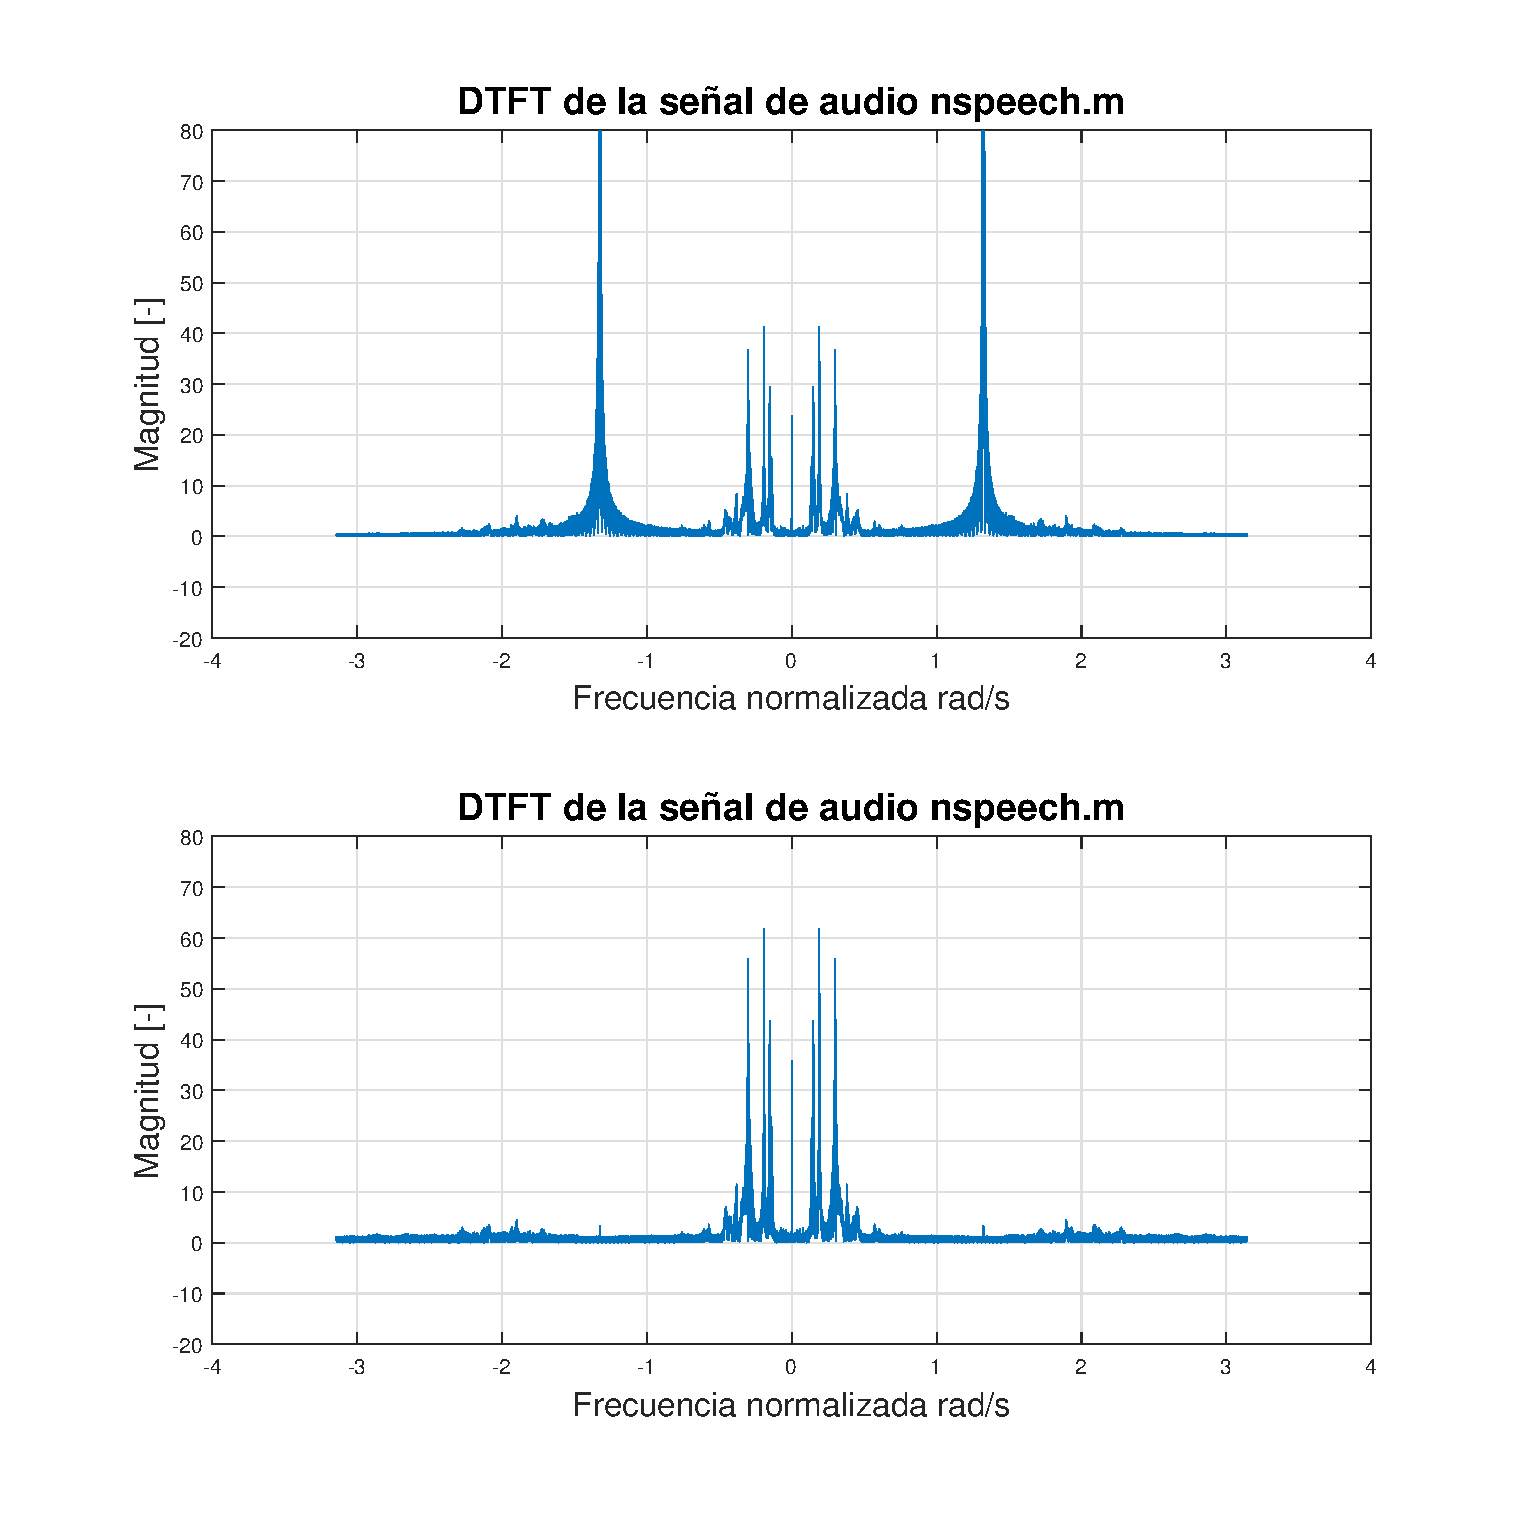
\includegraphics[scale = 0.4]{Figuras/p1_3-nspeech_filtrada.eps}
    \caption{Espectro en frecuencia del archivo \texttt{nspeech.mat} antes y después de ser filtrado.}
    \label{Fir}
\end{figure}

En donde se puede ver claramente que el tono puro que se encontraba en el archivo original se encuentra visualmente imperceptible luego de aplicar el filtro.

Cabe mencionar que el archivo original correspondía a un vector que contenía 13061 muestras, pero el resultado obtenido al aplicar la convolución con el filtro diseñado corresponde a un arreglo con tamaño distinto al original. Esto se debe a que para aplicar el comando de convolución \texttt{conv(u,v)} por lo que el tamaño del vector obtenido corresponde a $ \texttt{length(u)} + \texttt{length(b)} -1$ basado en  cómo se desarrolla el proceso de convolución.



\item Se busca filtrar el ruido presente en el archivo \texttt{pcm.mat} para lo que se diseña un filtro de tipo IIR. Se grafica el espectro en frecuencia de el archivo de audio para poder identificar cual es la frecuencia que contiene la  información que se desea conservar, esto se muestra en la gráfica de la figura \ref{dtft_pcm}

\begin{figure}[H]
    \centering
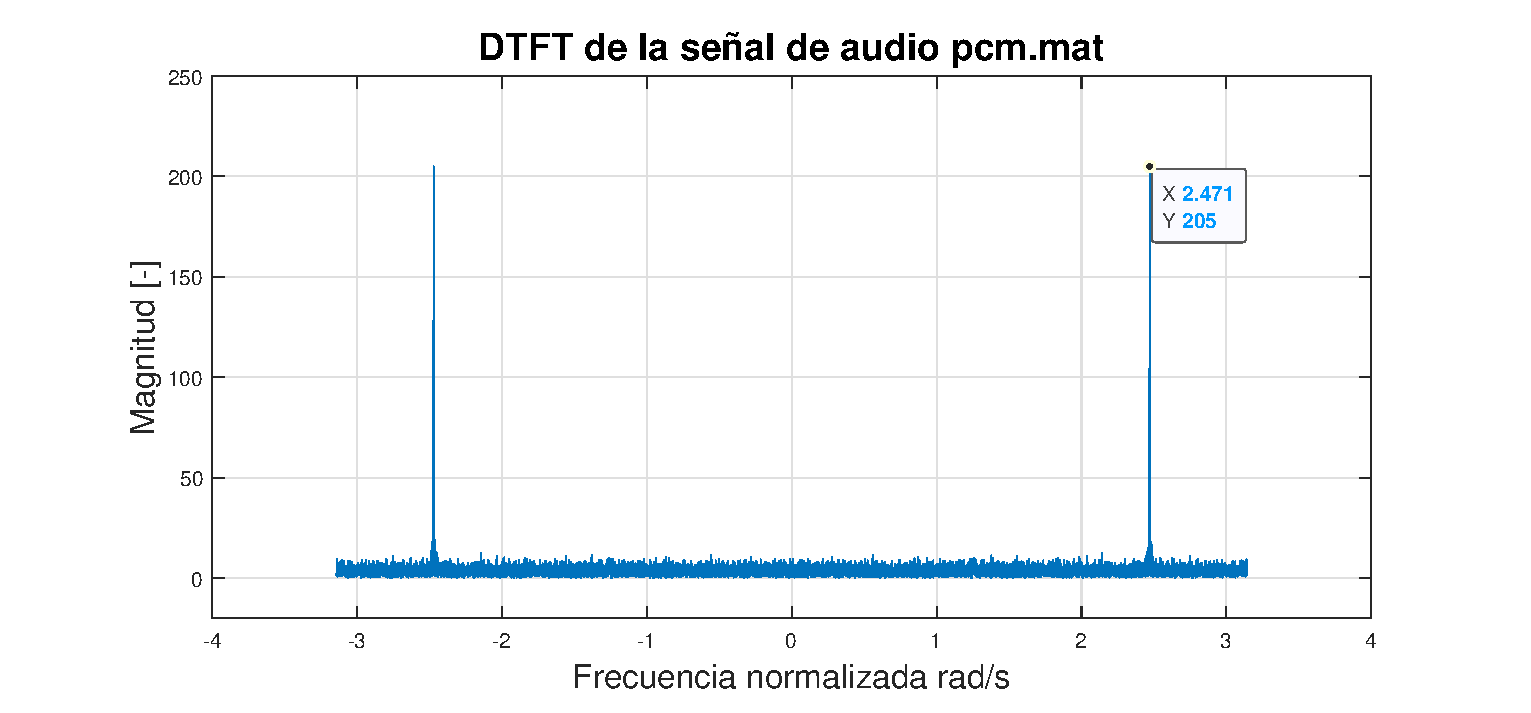
\includegraphics[scale = 0.6]{Figuras/p1_4-DTFT_pcm.eps}
    \caption{Espectro en frecuencia normalizada de \texttt{pcm.mat}.}
    \label{dtft_pcm}
\end{figure}

Donde se puede ver que el tono se encuentra en la frecuencia 1.323. Como la gráfica está en frecuencia normalizada, este valor corresponde al ángulo $\theta = 2.471$;


Se diseña entonces un filtro IIR con $r = 0.99$ y $\theta = 2.471$,  con función de transferencia

$$  H(z) = \frac{(1-r)z^2}{(z-re^{j\theta})(z-re^{-j\theta})} = \frac{(1-r)z^2}{z^2 -2~z~cos(\theta) + r^2}$$

Con coeficientes $a_k$

$$ a_k = [1 ~~-2cos(\theta) ~~ r^2]$$




Al implementar el filtro IIR mediante recurrencia, y aplicar el filtrado a la señal se obtienen los resultados presentes en las gráficas de la figura \ref{IIR}

\begin{figure}[H]
    \centering
    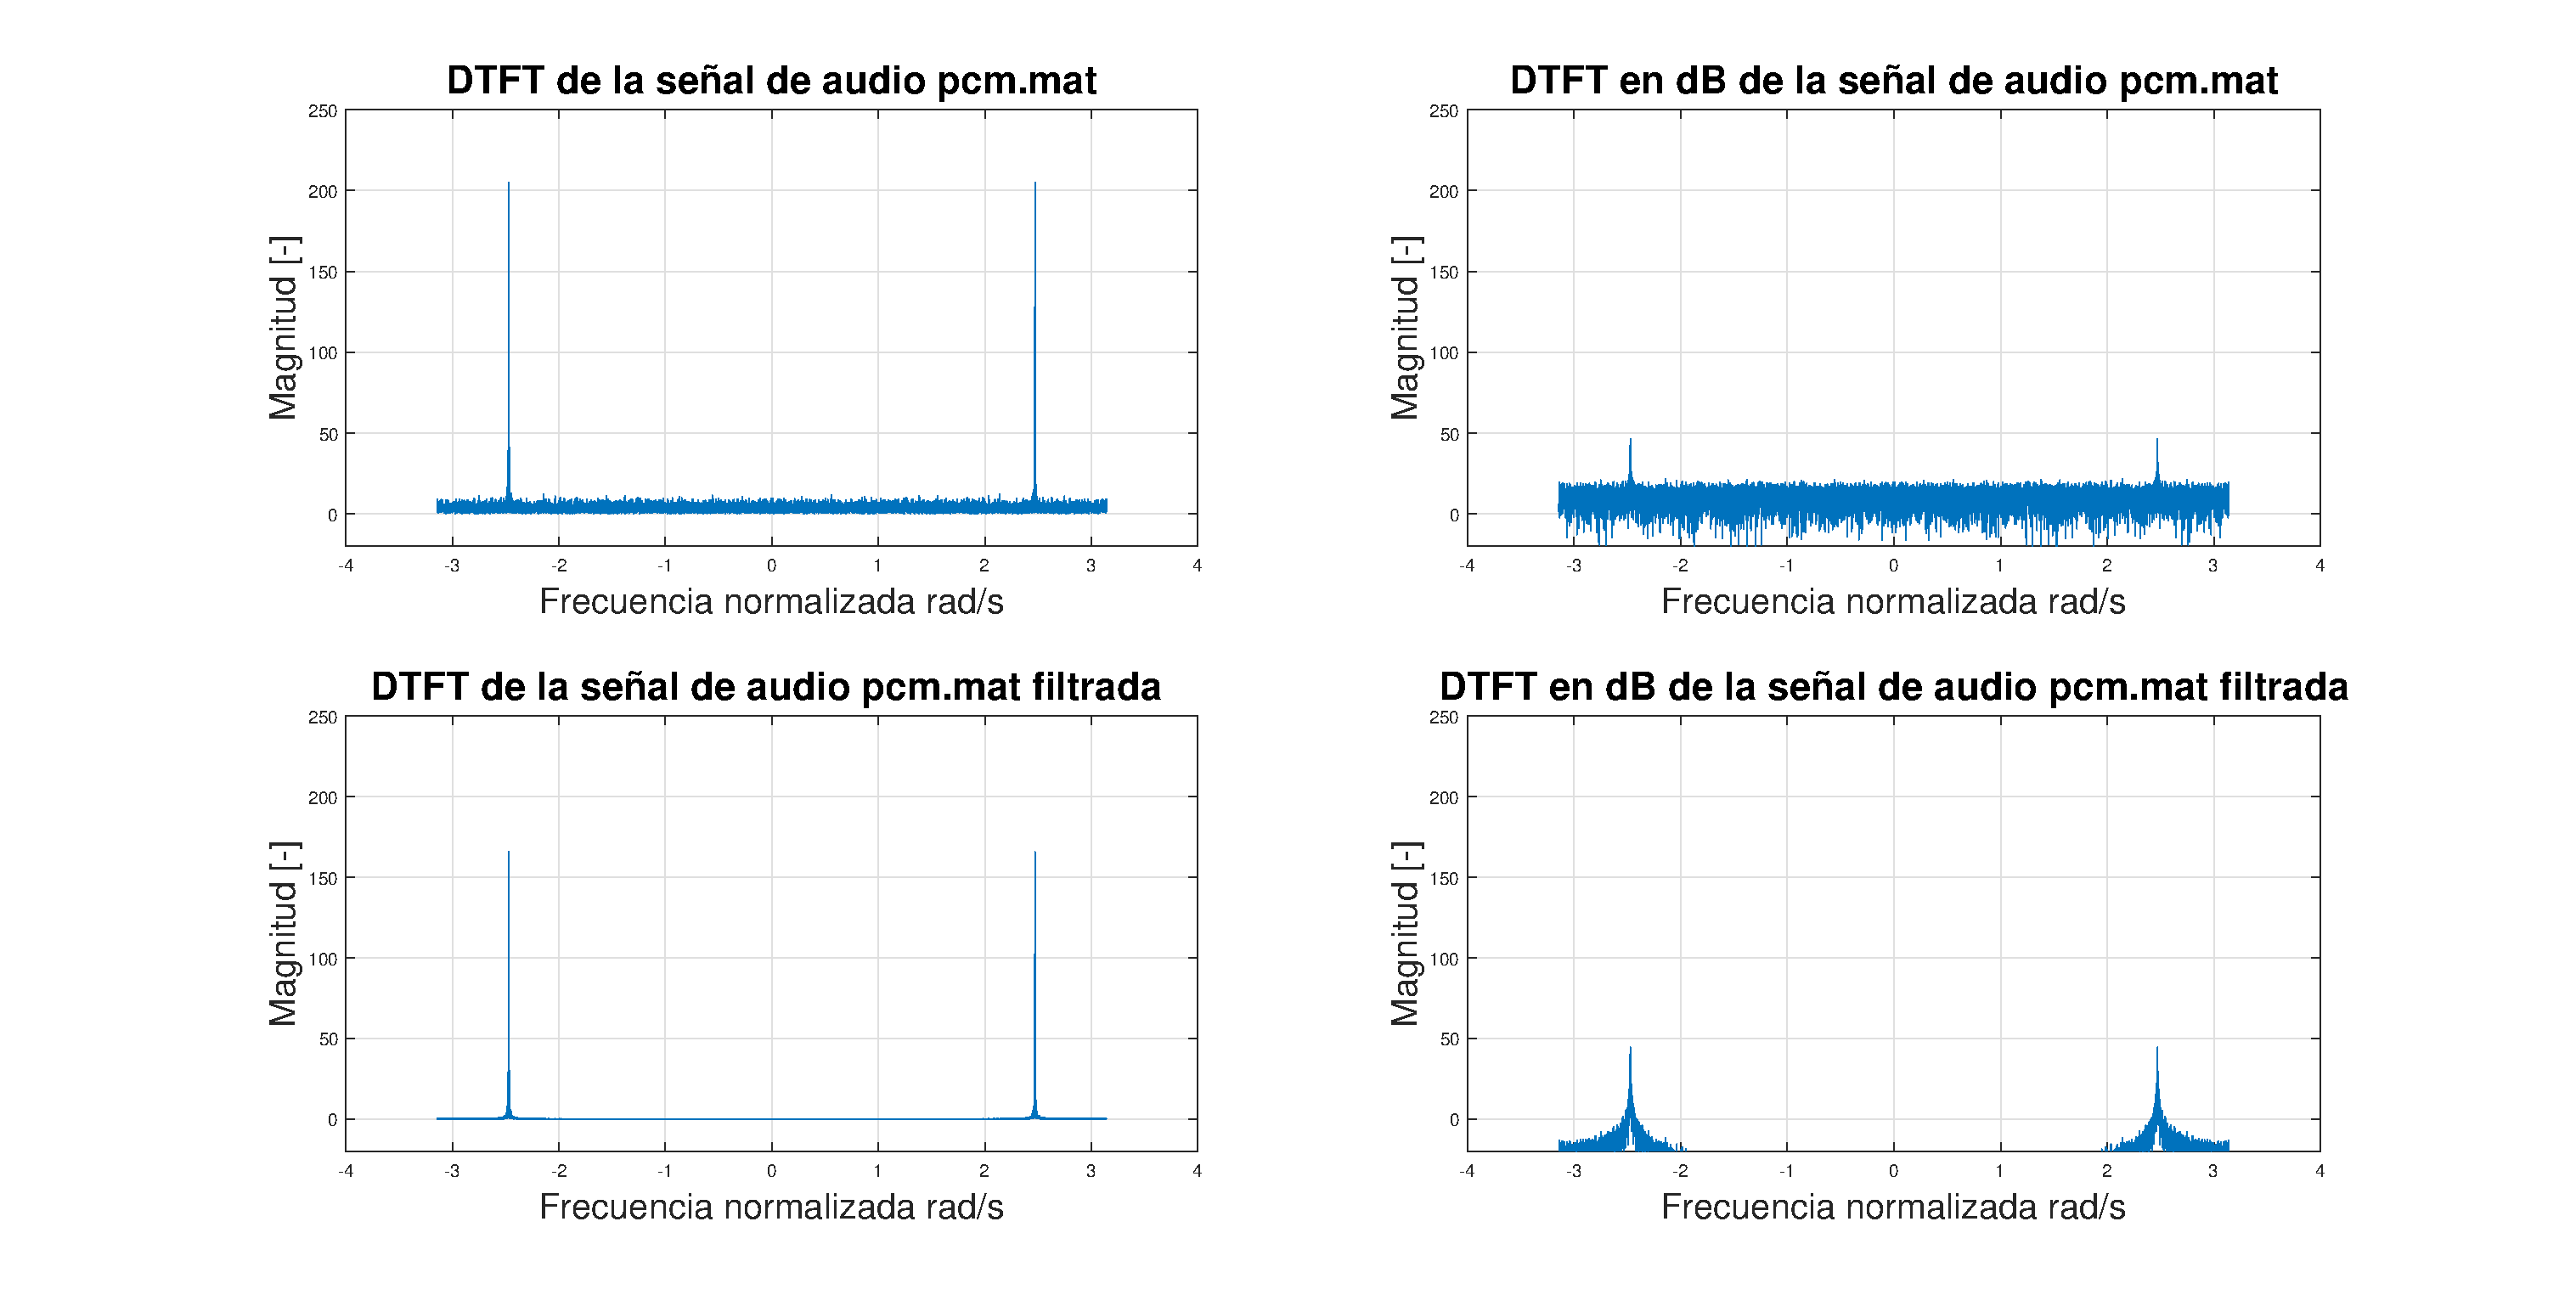
\includegraphics[scale = 0.3]{Figuras/p1_4-pcm_filtrada.eps}
    \caption{Espectro en frecuencia del archivo \texttt{pcm.mat} antes y después de ser filtrado.}
    \label{IIR}
\end{figure}


En la figura anterior se puede observar tanto en magnitud como en decibeles cómo se ha eliminado de forma significativa  el ruido presente en el archivo original.



